\documentclass[11pt]{article}
\usepackage{mathtools}
\usepackage{mdframed}
\usepackage{fullpage}
\usepackage{amsfonts}
\usepackage{tikz}
\usetikzlibrary{automata, positioning}



%edit this for each class
\newcommand\name{John Vincent}
\newcommand\classname{COMS 331}
\newcommand\assignment{Homework 2}



\newcounter{excounter}
\setcounter{excounter}{1}
\newcommand\question[2]{\vskip 1em  \noindent\textbf{\arabic{excounter}\addtocounter{excounter}{1}.} \emph{#1} \noindent#2}


% You can also erase this if you do not have package fancyhdr
% Fancy footnote.........
\usepackage{fancyhdr}  %% If it does not work with your latex installation, you may just delete this...
\pagestyle{fancy}
\usepackage{lastpage}
\rfoot{\name, page \thepage/\pageref{LastPage}}
\cfoot{}
\rhead{}
\lhead{}
\renewcommand{\headrulewidth}{0pt}
\renewcommand{\footrulewidth}{0pt}
\DeclarePairedDelimiter\ceil{\lceil}{\rceil}
\DeclarePairedDelimiter\floor{\lfloor}{\rfloor}



\begin{document}


  {\bf \classname \hspace{1cm} \assignment\hfill \name}
  \vskip 2em


  \question{}\\
  \hspace*{4.5cm}
  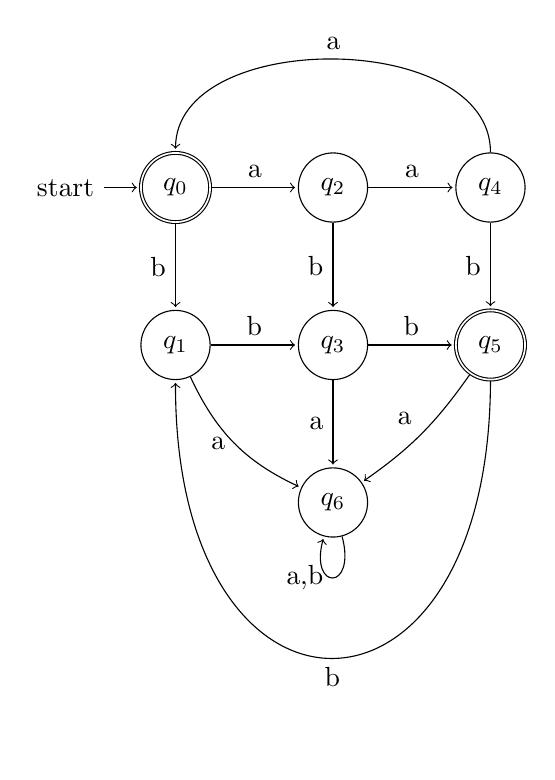
\begin{tikzpicture}[shorten >=1pt,node distance=2cm,on grid,auto]
   \node[state,initial,accepting] (q_0)   {$q_0$};
   \node[state] (q_1) [below=of q_0] {$q_1$};
   \node[state] (q_2) [right=of q_0] {$q_2$};
   \node[state](q_3) [below=of q_2] {$q_3$};
   \node[state](q_4) [right=of q_2] {$q_4$};
   \node[state, accepting](q_5) [below=of q_4] {$q_5$};
   \node[state](q_6) [below=of q_3] {$q_6$};
   \path[->]
   (q_0) edge node [above] {a} (q_2)
      edge node [left] {b} (q_1)
   (q_1) edge [bend right=20] node [left] {a} (q_6)
      edge node [above] {b} (q_3)
   (q_2) edge node [above] {a} (q_4)
      edge node [left] {b} (q_3)
   (q_3) edge node [left] {a} (q_6)
      edge node [above] {b} (q_5)
   (q_4) edge node [left] {b} (q_5)
   (q_4) edge [bend right=90] node [above] {a} (q_0)
   (q_5) edge [bend left=90, looseness=3] node [below] {b} (q_1)
      edge [bend left=10] node [above left] {a} (q_6)
   (q_6) edge [loop below] node [left] {a,b} ();
\end{tikzpicture}

\question{} this language accepts a binary string that has a 0 in the 8's place
\begin{center}
  $(0|1)^{*}0(0|1)(0|1)(0|1)$\\
  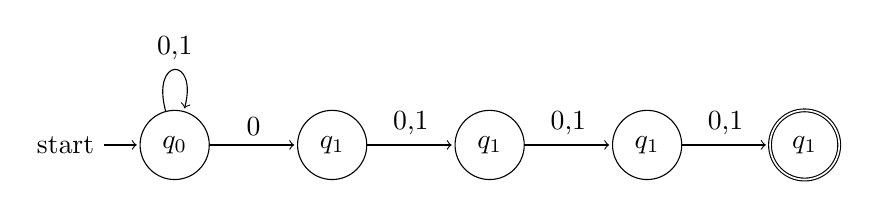
\begin{tikzpicture}[shorten >=1pt,node distance=2cm,on grid,auto]
    \node[state,initial] (q_0) {$q_0$};
    \node[state] (q_1) [right=of q_0] {$q_1$};
    \node[state] (q_2) [right=of q_1] {$q_1$};
    \node[state] (q_3) [right=of q_2] {$q_1$};
    \node[state, accepting] (q_4) [right=of q_3] {$q_1$};
    \path[->]
    (q_0) edge [loop above] node [above] {0,1} ()
      edge node [above] {0} (q_1)
    (q_1) edge node [above] {0,1} (q_2)
    (q_2) edge node [above] {0,1} (q_3)
    (q_3) edge node [above] {0,1} (q_4);
  \end{tikzpicture}
\end{center}
\clearpage
\question{}
\begin{center}
  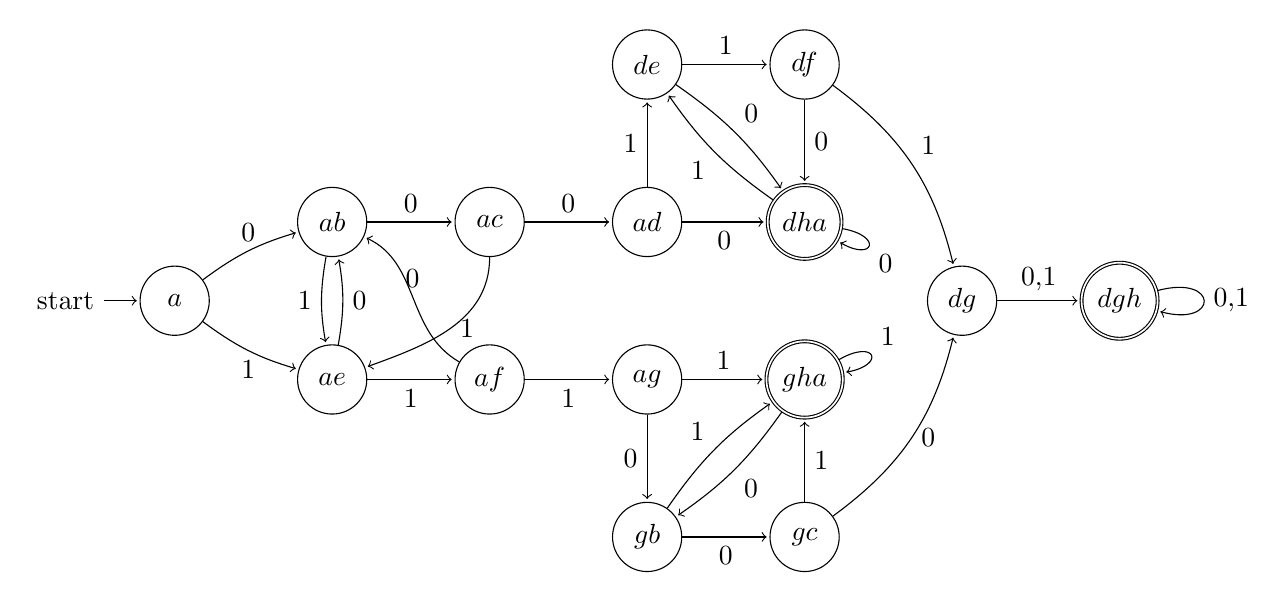
\begin{tikzpicture}[shorten >=1pt,node distance=2cm,on grid,auto]
    \node[state,initial] (q_0) {$a$};
    \node[state] (q_1) [above right= 1cm and 2cm of q_0] {$ab$};
    \node[state] (q_2) [below right= 1cm and 2cm of q_0] {$ae$};
    \node[state] (q_3) [right=of q_1] {$ac$};
    \node[state] (q_4) [right=of q_2] {$af$};
    \node[state] (q_5) [right=of q_3] {$ad$};
    \node[state] (q_6) [right=of q_4] {$ag$};
    \node[state, accepting] (q_7) [right=of q_5] {$dha$};
    \node[state, accepting] (q_8) [right=of q_6] {$gha$};
    \node[state] (q_9) [above=of q_5] {$de$};
    \node[state] (q_10) [below=of q_6] {$gb$};
    \node[state] (q_11) [right=of q_9] {$df$};
    \node[state] (q_12) [right=of q_10] {$gc$};
    \node[state] (q_13) [below right = 1cm and 2cm of q_7] {$dg$};
    \node[state,accepting] (q_14) [right= of q_13] {$dgh$};
    \path[->]
    (q_0) edge [bend left=10] node [above] {0} (q_1)
          edge [bend right=10] node [below] {1} (q_2)
    (q_1) edge node [above] {0} (q_3)
          edge [bend right=10] node [left] {1} (q_2)
    (q_2) edge node [below] {1} (q_4)
          edge [bend right=10] node [right] {0} (q_1)
    (q_3) edge node [above] {0} (q_5)
          edge [out=270, in=20] node [right] {1} (q_2)
    (q_4) edge node [below] {1} (q_6)
          edge [out=150, in=335] node [above] {0} (q_1)
    (q_5) edge node {1} (q_9)
          edge node [below] {0} (q_7)
    (q_6) edge node [left] {0} (q_10)
          edge node {1} (q_8)
    (q_7) edge [out=350, in=330,loop] node {0} ()
          edge [bend left=10] node {1} (q_9)
    (q_8) edge [out=30, in=10,loop] node {1} ()
          edge [bend left=10] node {0} (q_10)
    (q_9) edge [bend left=10] node {0} (q_7)
          edge node {1} (q_11)
    (q_10) edge [bend left=10] node {1} (q_8)
           edge node [below] {0} (q_12)
    (q_11) edge node {0} (q_7)
           edge [bend left= 20] node {1} (q_13)
    (q_12) edge node [right] {1} (q_8)
           edge [bend right= 20] node [right] {0} (q_13)
    (q_13) edge node {0,1} (q_14)
    (q_14) edge [loop right] node {0,1} ();
  \end{tikzpicture}
\end{center}

\end{document}
